\section{Natural Deduction}

\subsection{Natural deduction}

The Lean proofs for this chapter live in
\href{/NaturalDeduction-2aa9a550d0740195b99b61fcb067c242.lean}{\texttt{LearningLean/NaturalDeduction.lean}}, inside the
\texttt{Exercises} namespace.

\subsubsection{5.5 Reduction to the absurd. $P \Rightarrow Q,\ ¬ Q ⊢ ¬ P$}

This is a very useful technique. Validity of
$P \Rightarrow Q,\ ¬ Q ⊢ ¬ P$ is proved with:

\begin{figure}[!htbp]
\centering
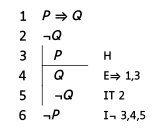
\includegraphics[width=0.4\linewidth]{files/fitch-b1b30d3bae99cd633d830976f12fffdb.svg}
\end{figure}

The sub-derivation (lines 3--5) discharges the hypothesis $P$: assuming $P$,
[$\Rightarrow$-elimination] on lines 1 and 3 gives $Q$, while line 2 reiterates
$¬ Q$. The contradiction lets us introduce $¬ P$ ($¬$-introduction over
lines 3, 4, 5).

In Lean this is theorem \texttt{T55}, where \texttt{¬P} is definitionally \texttt{P \rightarrow False},\footnote{This is the standard definition in Lean's core library: \texttt{Not p} unfolds to \texttt{p \rightarrow False},
so a proof of \texttt{¬P} is exactly a function turning a proof of \texttt{P} into a proof of \texttt{False}.} so the
whole proof is just function composition:

\begin{verbatim}
theorem T55 (h1 : P \rightarrow Q) (h2 : ¬Q) : ¬P :=
  (h2 ∘ h1)
\end{verbatim}

\subsubsection{Conjunction introduction. $P,\ P \Rightarrow Q ⊢ P \wedge Q$}

Theorem \texttt{T51} builds the pair \texttt{⟨proof of P, proof of Q⟩} directly, using the
anonymous-constructor notation \texttt{⟨\_, \_⟩}:

\begin{verbatim}
theorem T51 (h1 : P) (h2 : P \rightarrow Q) : P ∧ Q :=
  ⟨h1, h2 h1⟩
\end{verbatim}